\documentclass[tikz,border=10pt]{standalone}
\usepackage{tikz}

\begin{document}
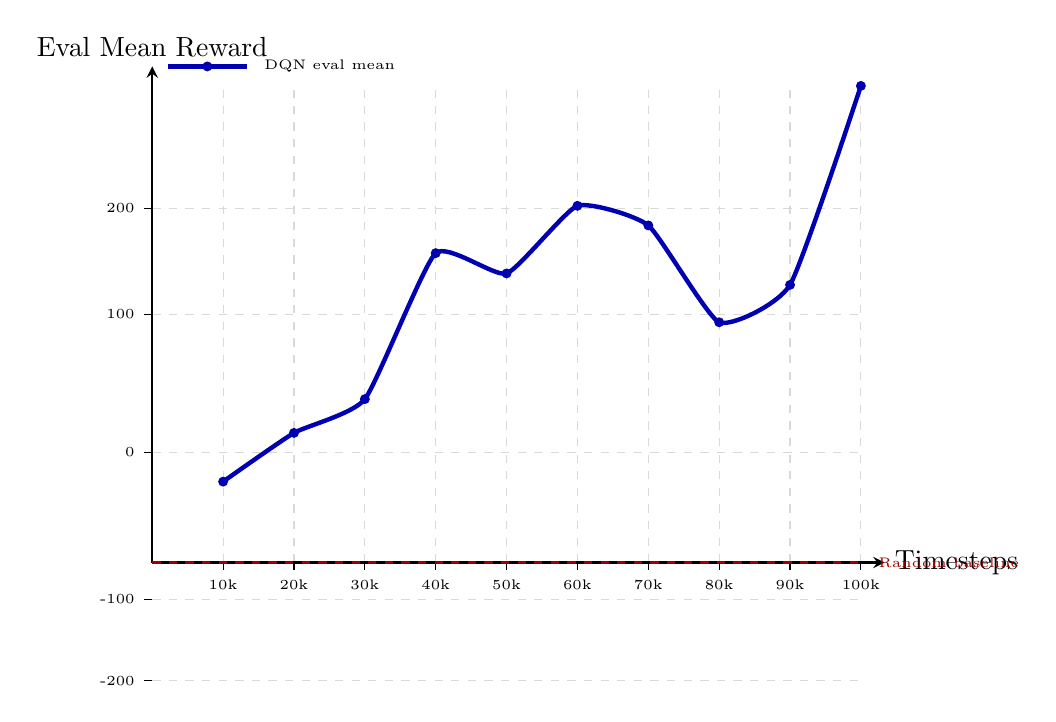
\begin{tikzpicture}[>=stealth,scale=1.0]

% Origin
\def\ox{1.0}
\def\oy{-1.5}
\def\xw{9.0}
\def\yh{6.0}

% Pre-computed y-positions for grid lines
\def\yA{-1.500}  % -200 -> bottom
\def\yB{-0.466}  % -100
\def\yC{1.397}   % 0
\def\yD{3.155}   % 100
\def\yE{4.500}   % 200 -> top

% Horizontal grid + labels
\draw[gray!30,dashed] (\ox,\oy+\yA) -- (\ox+\xw,\oy+\yA);
\draw (\ox,\oy+\yA) -- (\ox-0.1,\oy+\yA); \node[left,font=\tiny] at (\ox-0.1,\oy+\yA) {-200};

\draw[gray!30,dashed] (\ox,\oy+\yB) -- (\ox+\xw,\oy+\yB);
\draw (\ox,\oy+\yB) -- (\ox-0.1,\oy+\yB); \node[left,font=\tiny] at (\ox-0.1,\oy+\yB) {-100};

\draw[gray!30,dashed] (\ox,\oy+\yC) -- (\ox+\xw,\oy+\yC);
\draw (\ox,\oy+\yC) -- (\ox-0.1,\oy+\yC); \node[left,font=\tiny] at (\ox-0.1,\oy+\yC) {0};

\draw[gray!30,dashed] (\ox,\oy+\yD) -- (\ox+\xw,\oy+\yD);
\draw (\ox,\oy+\yD) -- (\ox-0.1,\oy+\yD); \node[left,font=\tiny] at (\ox-0.1,\oy+\yD) {100};

\draw[gray!30,dashed] (\ox,\oy+\yE) -- (\ox+\xw,\oy+\yE);
\draw (\ox,\oy+\yE) -- (\ox-0.1,\oy+\yE); \node[left,font=\tiny] at (\ox-0.1,\oy+\yE) {200};

% Vertical grid + labels
\draw[gray!30,dashed] (\ox+0.900,\oy) -- (\ox+0.900,\oy+\yh);
\draw (\ox+0.900,\oy) -- (\ox+0.900,\oy-0.1); \node[below,font=\tiny] at (\ox+0.900,\oy-0.1) {10k};

\draw[gray!30,dashed] (\ox+1.800,\oy) -- (\ox+1.800,\oy+\yh);
\draw (\ox+1.800,\oy) -- (\ox+1.800,\oy-0.1); \node[below,font=\tiny] at (\ox+1.800,\oy-0.1) {20k};

\draw[gray!30,dashed] (\ox+2.700,\oy) -- (\ox+2.700,\oy+\yh);
\draw (\ox+2.700,\oy) -- (\ox+2.700,\oy-0.1); \node[below,font=\tiny] at (\ox+2.700,\oy-0.1) {30k};

\draw[gray!30,dashed] (\ox+3.600,\oy) -- (\ox+3.600,\oy+\yh);
\draw (\ox+3.600,\oy) -- (\ox+3.600,\oy-0.1); \node[below,font=\tiny] at (\ox+3.600,\oy-0.1) {40k};

\draw[gray!30,dashed] (\ox+4.500,\oy) -- (\ox+4.500,\oy+\yh);
\draw (\ox+4.500,\oy) -- (\ox+4.500,\oy-0.1); \node[below,font=\tiny] at (\ox+4.500,\oy-0.1) {50k};

\draw[gray!30,dashed] (\ox+5.400,\oy) -- (\ox+5.400,\oy+\yh);
\draw (\ox+5.400,\oy) -- (\ox+5.400,\oy-0.1); \node[below,font=\tiny] at (\ox+5.400,\oy-0.1) {60k};

\draw[gray!30,dashed] (\ox+6.300,\oy) -- (\ox+6.300,\oy+\yh);
\draw (\ox+6.300,\oy) -- (\ox+6.300,\oy-0.1); \node[below,font=\tiny] at (\ox+6.300,\oy-0.1) {70k};

\draw[gray!30,dashed] (\ox+7.200,\oy) -- (\ox+7.200,\oy+\yh);
\draw (\ox+7.200,\oy) -- (\ox+7.200,\oy-0.1); \node[below,font=\tiny] at (\ox+7.200,\oy-0.1) {80k};

\draw[gray!30,dashed] (\ox+8.100,\oy) -- (\ox+8.100,\oy+\yh);
\draw (\ox+8.100,\oy) -- (\ox+8.100,\oy-0.1); \node[below,font=\tiny] at (\ox+8.100,\oy-0.1) {90k};

\draw[gray!30,dashed] (\ox+9.000,\oy) -- (\ox+9.000,\oy+\yh);
\draw (\ox+9.000,\oy) -- (\ox+9.000,\oy-0.1); \node[below,font=\tiny] at (\ox+9.000,\oy-0.1) {100k};

% Axes
\draw[->,thick] (\ox,\oy) -- (\ox+\xw+0.3,\oy) node[right] {Timesteps};
\draw[->,thick] (\ox,\oy) -- (\ox,\oy+\yh+0.3) node[above] {Eval Mean Reward};

% Random baseline
\draw[red!60!black,dashed,thick] (\ox,\oy) -- (\ox+\xw,\oy);
\node[red!60!black,font=\tiny,right] at (\ox+\xw+0.1,\oy) {Random baseline};

% Data points (pre-computed: x=ox+0.9 to ox+9.0, y=oy+(ydata+280)/580*6)
\coordinate (p1) at (1.900,-0.473);
\coordinate (p2) at (2.800,0.146);
\coordinate (p3) at (3.700,0.575);
\coordinate (p4) at (4.600,2.429);
\coordinate (p5) at (5.500,2.171);
\coordinate (p6) at (6.400,3.030);
\coordinate (p7) at (7.300,2.781);
\coordinate (p8) at (8.200,1.551);
\coordinate (p9) at (9.100,2.026);
\coordinate (p10) at (10.000,4.553);

% Smooth line
\draw[blue!70!black,ultra thick,smooth] plot[smooth,tension=0.3] coordinates {(p1) (p2) (p3) (p4) (p5) (p6) (p7) (p8) (p9) (p10)};

% Points
\fill[blue!70!black] (p1) circle (1.8pt);
\fill[blue!70!black] (p2) circle (1.8pt);
\fill[blue!70!black] (p3) circle (1.8pt);
\fill[blue!70!black] (p4) circle (1.8pt);
\fill[blue!70!black] (p5) circle (1.8pt);
\fill[blue!70!black] (p6) circle (1.8pt);
\fill[blue!70!black] (p7) circle (1.8pt);
\fill[blue!70!black] (p8) circle (1.8pt);
\fill[blue!70!black] (p9) circle (1.8pt);
\fill[blue!70!black] (p10) circle (1.8pt);

% Legend
\draw[blue!70!black,ultra thick] (1.2,4.8) -- (2.2,4.8);
\fill[blue!70!black] (1.7,4.8) circle (1.8pt);
\node[right,font=\tiny] at (2.3,4.8) {DQN eval mean};

\end{tikzpicture}
\end{document}
